
\documentclass[twoside,onecolumn]{article}

\usepackage{blindtext} % Package to generate dummy text throughout this template 

%\usepackage[sc]{mathpazo} % Use the Palatino font
\usepackage[T1]{fontenc} % Use 8-bit encoding that has 256 glyphs
\linespread{1.05} % Line spacing - Palatino needs more space between lines
\usepackage{microtype} % Slightly tweak font spacing for aesthetics
\usepackage{float}
 \usepackage{amsmath}
 \usepackage{booktabs}
 \usepackage{amssymb}
 \usepackage{amsthm}
 \usepackage{tabularx} %tabelle
 \usepackage{tikz} %circuiti
 \usepackage{enumerate}
 \usepackage{pgfplots}
 \usepackage{subcaption}
\usepackage[toc,page]{appendix}
 \usepackage[export]{adjustbox}
 \usepackage{caption}
 \usepackage{subfig}
 \usepackage{sidecap}
 \usepackage{graphicx}
 \theoremstyle{definition}
  \usepackage{multicol}
  \usetikzlibrary{arrows}
  
\usepackage[english]{babel} % Language hyphenation and typographical rules

\usepackage[hmarginratio=1:1,top=32mm,columnsep=20pt]{geometry} % Document margins
\usepackage[hang, small,labelfont=bf,up,textfont=it,up]{caption} % Custom captions under/above floats in tables or figures
\usepackage{booktabs} % Horizontal rules in tables

\usepackage{lettrine} % The lettrine is the first enlarged letter at the beginning of the text

\usepackage{enumitem} % Customized lists
\setlist[itemize]{noitemsep} % Make itemize lists more compact

\usepackage{titlesec} % Allows customization of titles
\titleformat{\section}[block]{\large\scshape\centering}{\thesection.}{1em}{} % Change the look of the section titles
\titleformat{\subsection}[block]{\large}{\thesubsection.}{1em}{} % Change the look of the section titles

\usepackage{hyperref} % For hyperlinks in the PDF

\title{Homework 1: Summarizing Performance Data } % Article title
\author{Nicole Zattarin}
\date{} 
\begin{document}

% Print the title
\maketitle

\begin{abstract}
In order to draw significant information about the obtained results, every simulation must be supported with a rigorous data analysis. Therefore, being able to study in a proper and theoretically rigorous way the statistical properties of a dataset is a fundamental skill required for scientific simulation. This report first explores different tools and then test them on two simple simulations of randomly generated  data.
\end{abstract}



\section{Comparing data: the example of two operating systems}

\subsection{Display distributions}

Let us consider the example of two operating systems: an older one and its new version, whose performances are supposed to be better. We want to explore different visualization and statistical tools that allow to compare performances. To this end, we are going to deal with data regarding the execution times of a series of commonly used programs with both options.

\begin{figure}\centering
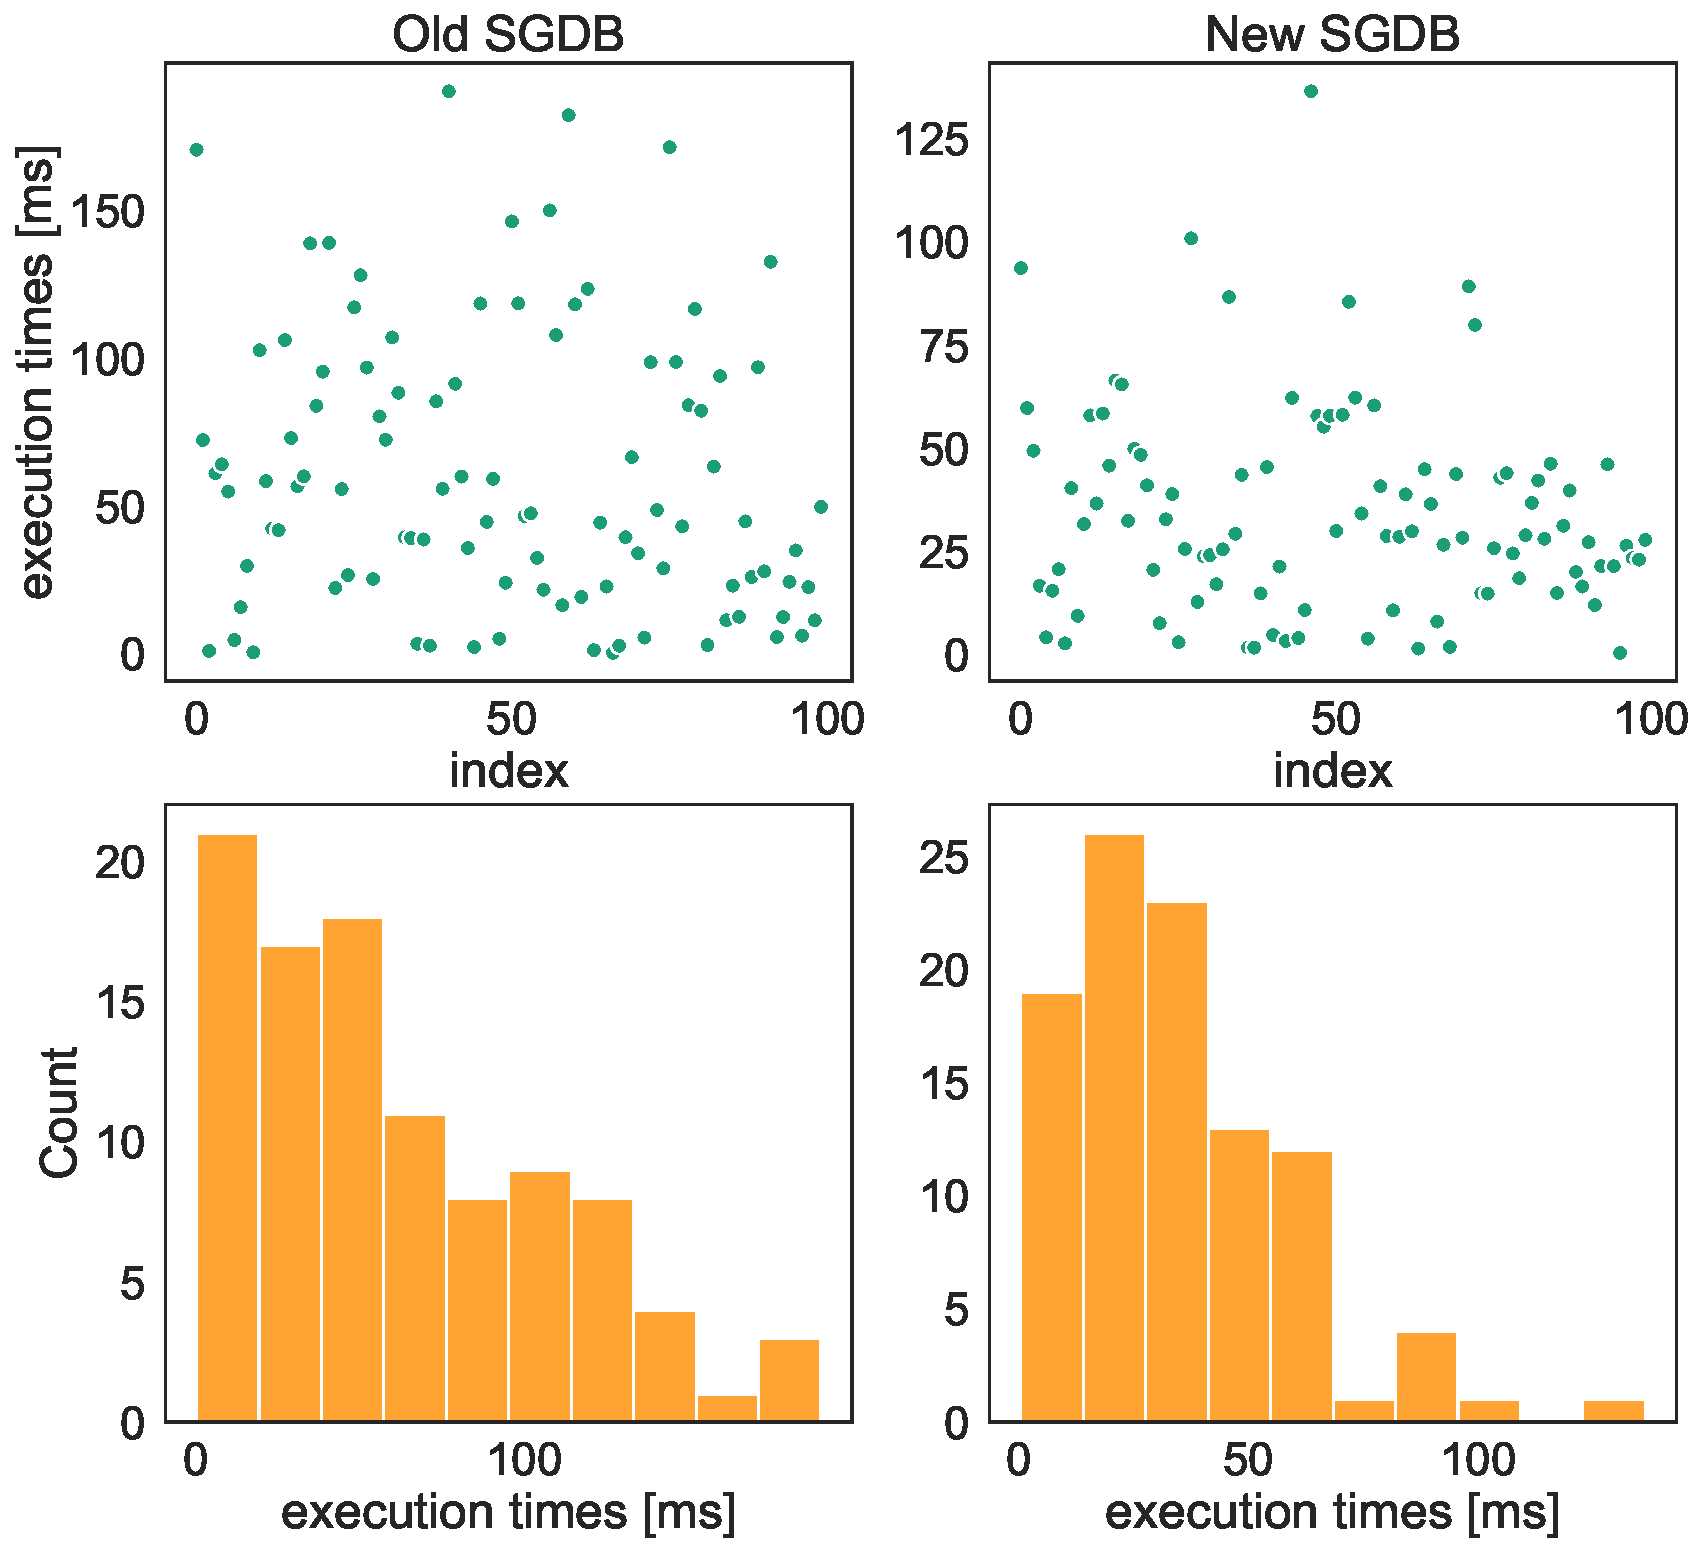
\includegraphics[width=0.8\textwidth]{../figs/extimes_distributions_vs_scatter.pdf}
\caption{Measured execution times in ms for 100 transactions with the old (left) and new (right) systems. Upper panels represents the scatterplot, while lower panels exhibit the distribution od data by means of histograms. }\label{fig:distribution_scatter}
\end{figure}


 \par
In Figure \ref{fig:distribution_scatter} we report both the distributions and the individual data for each of the two versions. It is possible to highlight that the histograms provide informations regarding the statistical distributions of data, while scatterplots allow us only to individuate a qualitative trend in the observed data. Therefore, a more quantitative way to extrapolate information is needed. A good option consist of comparing the cumulative density functions of the two distributions, in Figure \ref{fig:cdf} we report the CDF for both the versions of the operating system. Since the CDF corresponding to the run times of the new systems is almost constantly above the other one, we can conclude that the new approach is better performing than the previous one.\\Finally, it may be useful to compare two distributions by means of boxplots, swarmplots and violinplots, in Figure \ref{fig:boxswarm} we provide both boxplots and swarmplots of each of the two distributions. Such tools are particularly useful to represent quantiles and, for what concerns violinplots and swarmplots, a qualitative shape of the distribution.


\begin{figure}\centering
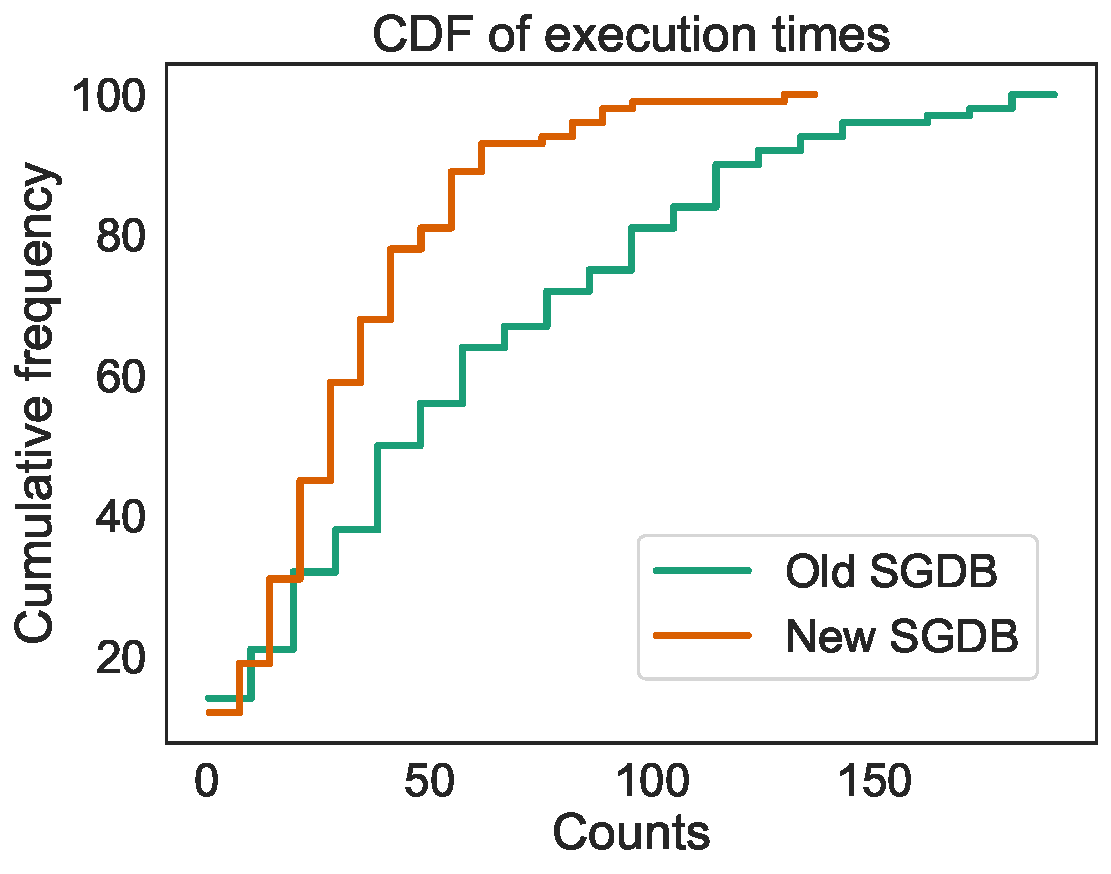
\includegraphics[width=0.5\textwidth]{../figs/extimes_CDF.pdf}
\caption{Cumulative density functions of the distribution of run times for both the systems considered. }\label{fig:cdf}
\end{figure}

\begin{figure}\centering
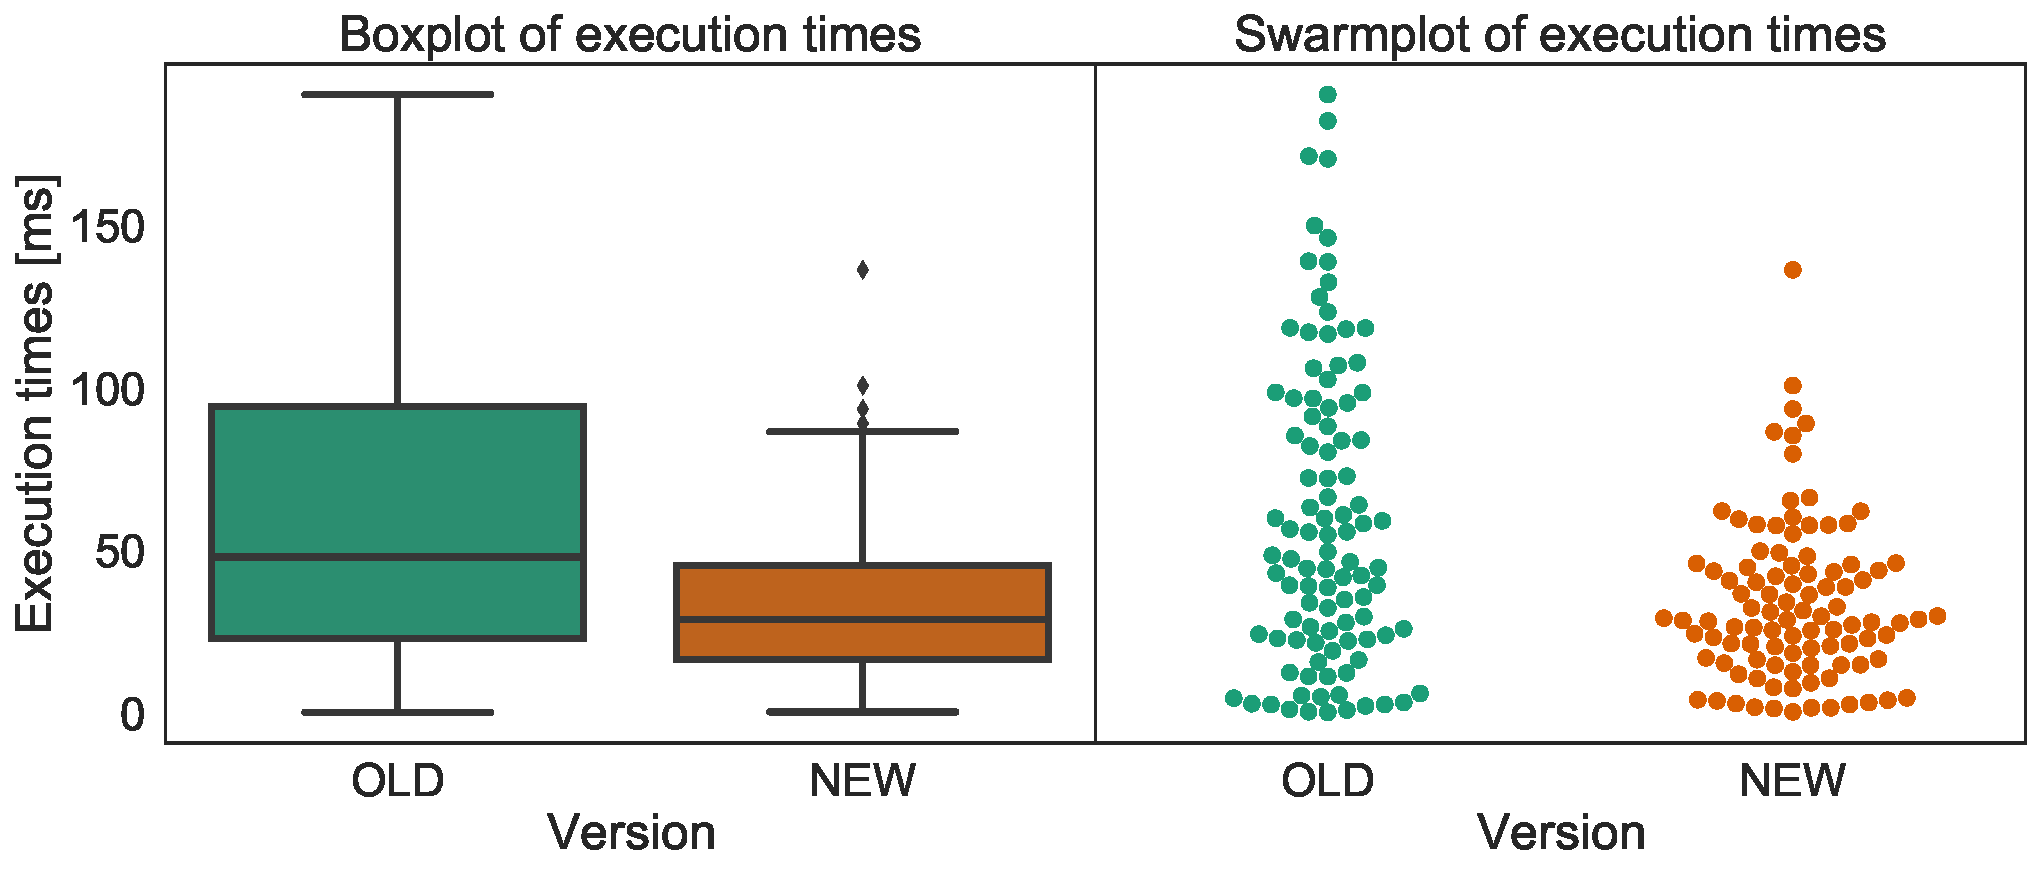
\includegraphics[width=0.9
\textwidth]{../figs/extimes_quantiles.pdf}
\caption{Quantiles of the execution times concerning both the old and new system. Left panel shows the boxplots, while right panel exhibits swarmplots.}\label{fig:boxswarm}
\end{figure}


\subsection{Confidence intervals}
Moreover, we could be interested in comparing the two versions by defining a quantitative measure of the improvement due to the new system. A possible way to be quantitative  consist of measuring the reduction in run time for the same sequence of tasks. In Figure \ref{fig:reduction}, the first panel shows the scatterplot of reductions in running time, the second exhibits the confidence intervals for the mean and for the median, while the right panel represents the distribution of reductions.

\begin{figure} \centering
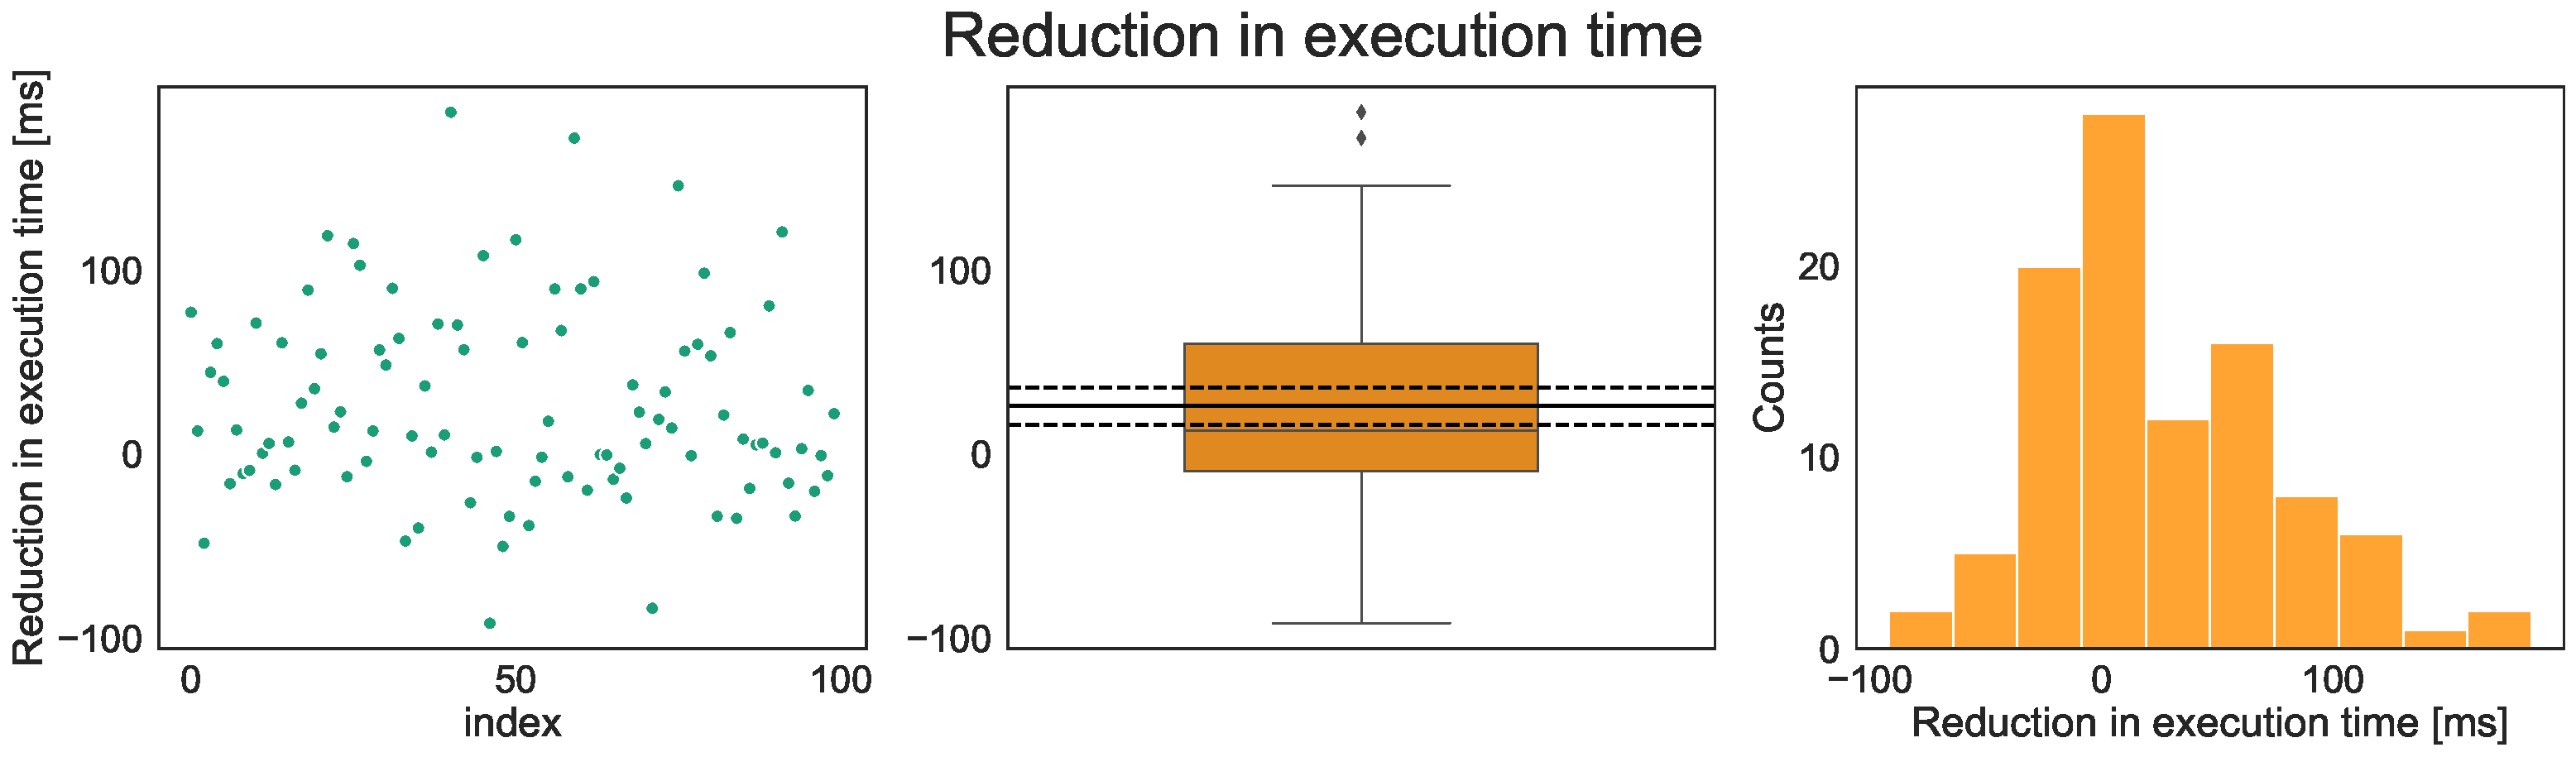
\includegraphics[width=1\textwidth]{../figs/extimes_reduction.pdf}
\caption{Different visualizations of the reduction times in ms from the older to the more recent version of the operating system. Right panel shows the scatterplot relative to individual data, while right panel shows the distribution. The central plot shows the quantile and the mean (horizontal line), with its confidence interval (dashed lines).}\label{fig:reduction}
\end{figure}

Nevertheless, it is worth to highlight that the theory provides different methods to compute confidence intervals for the mean. We already exploited the standard one to compute the CI of the run time reductions, but two more approaches can be investigated: one relies on the assumption that data are normally distributed, while the second is known as bootstrap method. In Figure \ref{fig:ci_methods} we show mean CI for all the methods proposed, both for the new and the old system.
All computations are carried out assuming a confidence level of 0.95.

\begin{figure} \centering
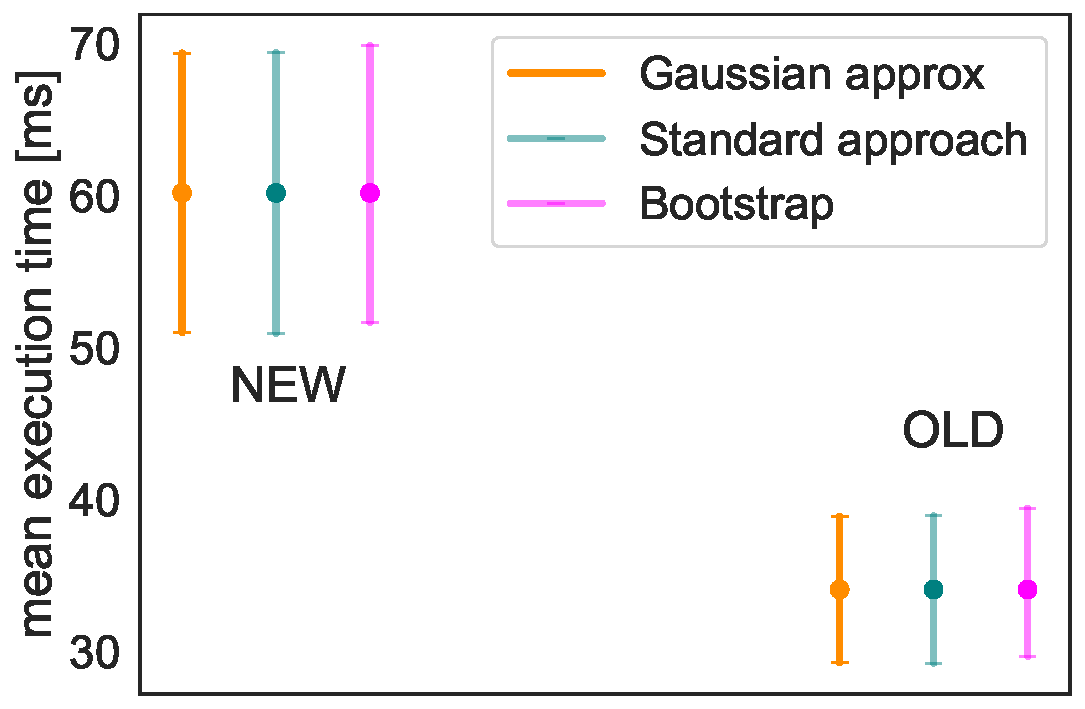
\includegraphics[width=0.5\textwidth]{../figs/CI_methods_comparison.pdf}
\caption{Confidence intervals of mean reduction times for the old and the new version, computation is carried out with different methods. Results show that the mean execution time of the new version is better than the older, while different methods provide similar outcomes.}\label{fig:ci_methods}
\end{figure}

\begin{figure} \centering
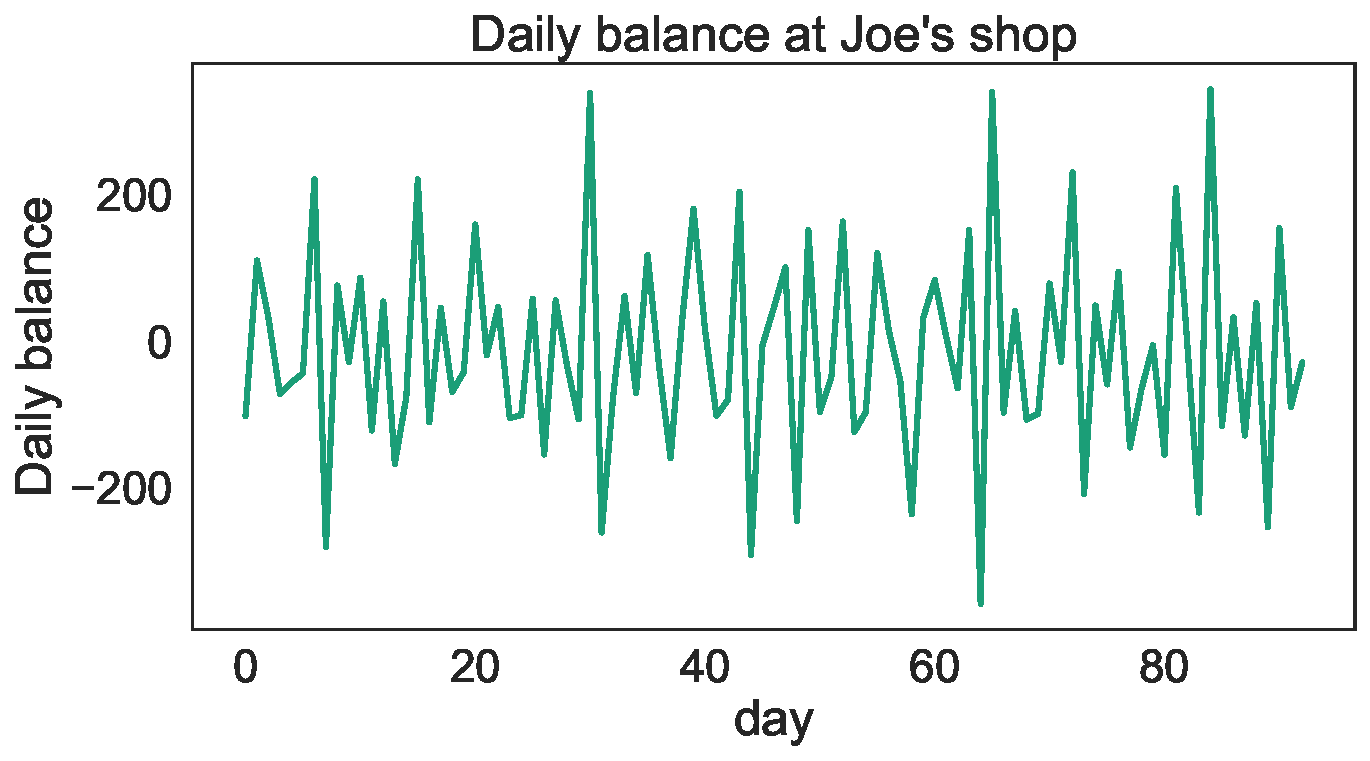
\includegraphics[width=0.7\textwidth]{../figs/joe_lineplot.pdf}
\caption{The time evolution of the daily balance provides qualitative informations about the trend, but it does not allow to determine if data are iid.}\label{fig:lineplot_joe}
\end{figure}

\section{Time series:the example of daily balance data}
Let us consider an example of time series, in order to explore some useful tools.
We consider data coming from a shop: at the end of day $t-1$ the amount of cash in the register is $c_{t-1}$, employees count it and puts it into the safe. The next day, $c_{t-1}$ is returned to the cash register, thus at the end of the day $c_t$ is equal to $c_{t-1}$, plus the profit of the day $s_t$, minus the amount of cash sent to the bank $b_t$. Therefore, we get $c_t=c_{t-1}+s_t-b_t$. Nevertheless, in practice this is subjected to error, we study the daily evolution of such error, to whom we refer as daily balance, $Y=c_t-c_{t-1}-s_t+b_t$.

To observe the qualitative trend of data, in Figure \ref{fig:lineplot_joe} we exhibit the time evolution of balance. Even though, it is worth to highlight that it is not possible to discriminate if the dataset consists of $iid$ items just having a look at time evolution. Since we are interested in studying if the balance of a certain day depends on the previous days, we consider log plots, which are scatterplots of the data at time $t$ versus the shifted data at time $t+h$, for different values of $h$. In Figure \ref{fig:joe_lag_plots} we exhibit log plots for different values of $h$: it is clear that there is a strong correlation with the previous day, even tough correlations decrease as we consider higher values of h, i.e. larger time shifts. Finally, another interesting approach to individuate correlations in a time serie is to study the autocorrelation plot: it provides the correlation coefficient between $y(t)$ and $y(t+h)$ for different shifts. 

\begin{figure} \centering
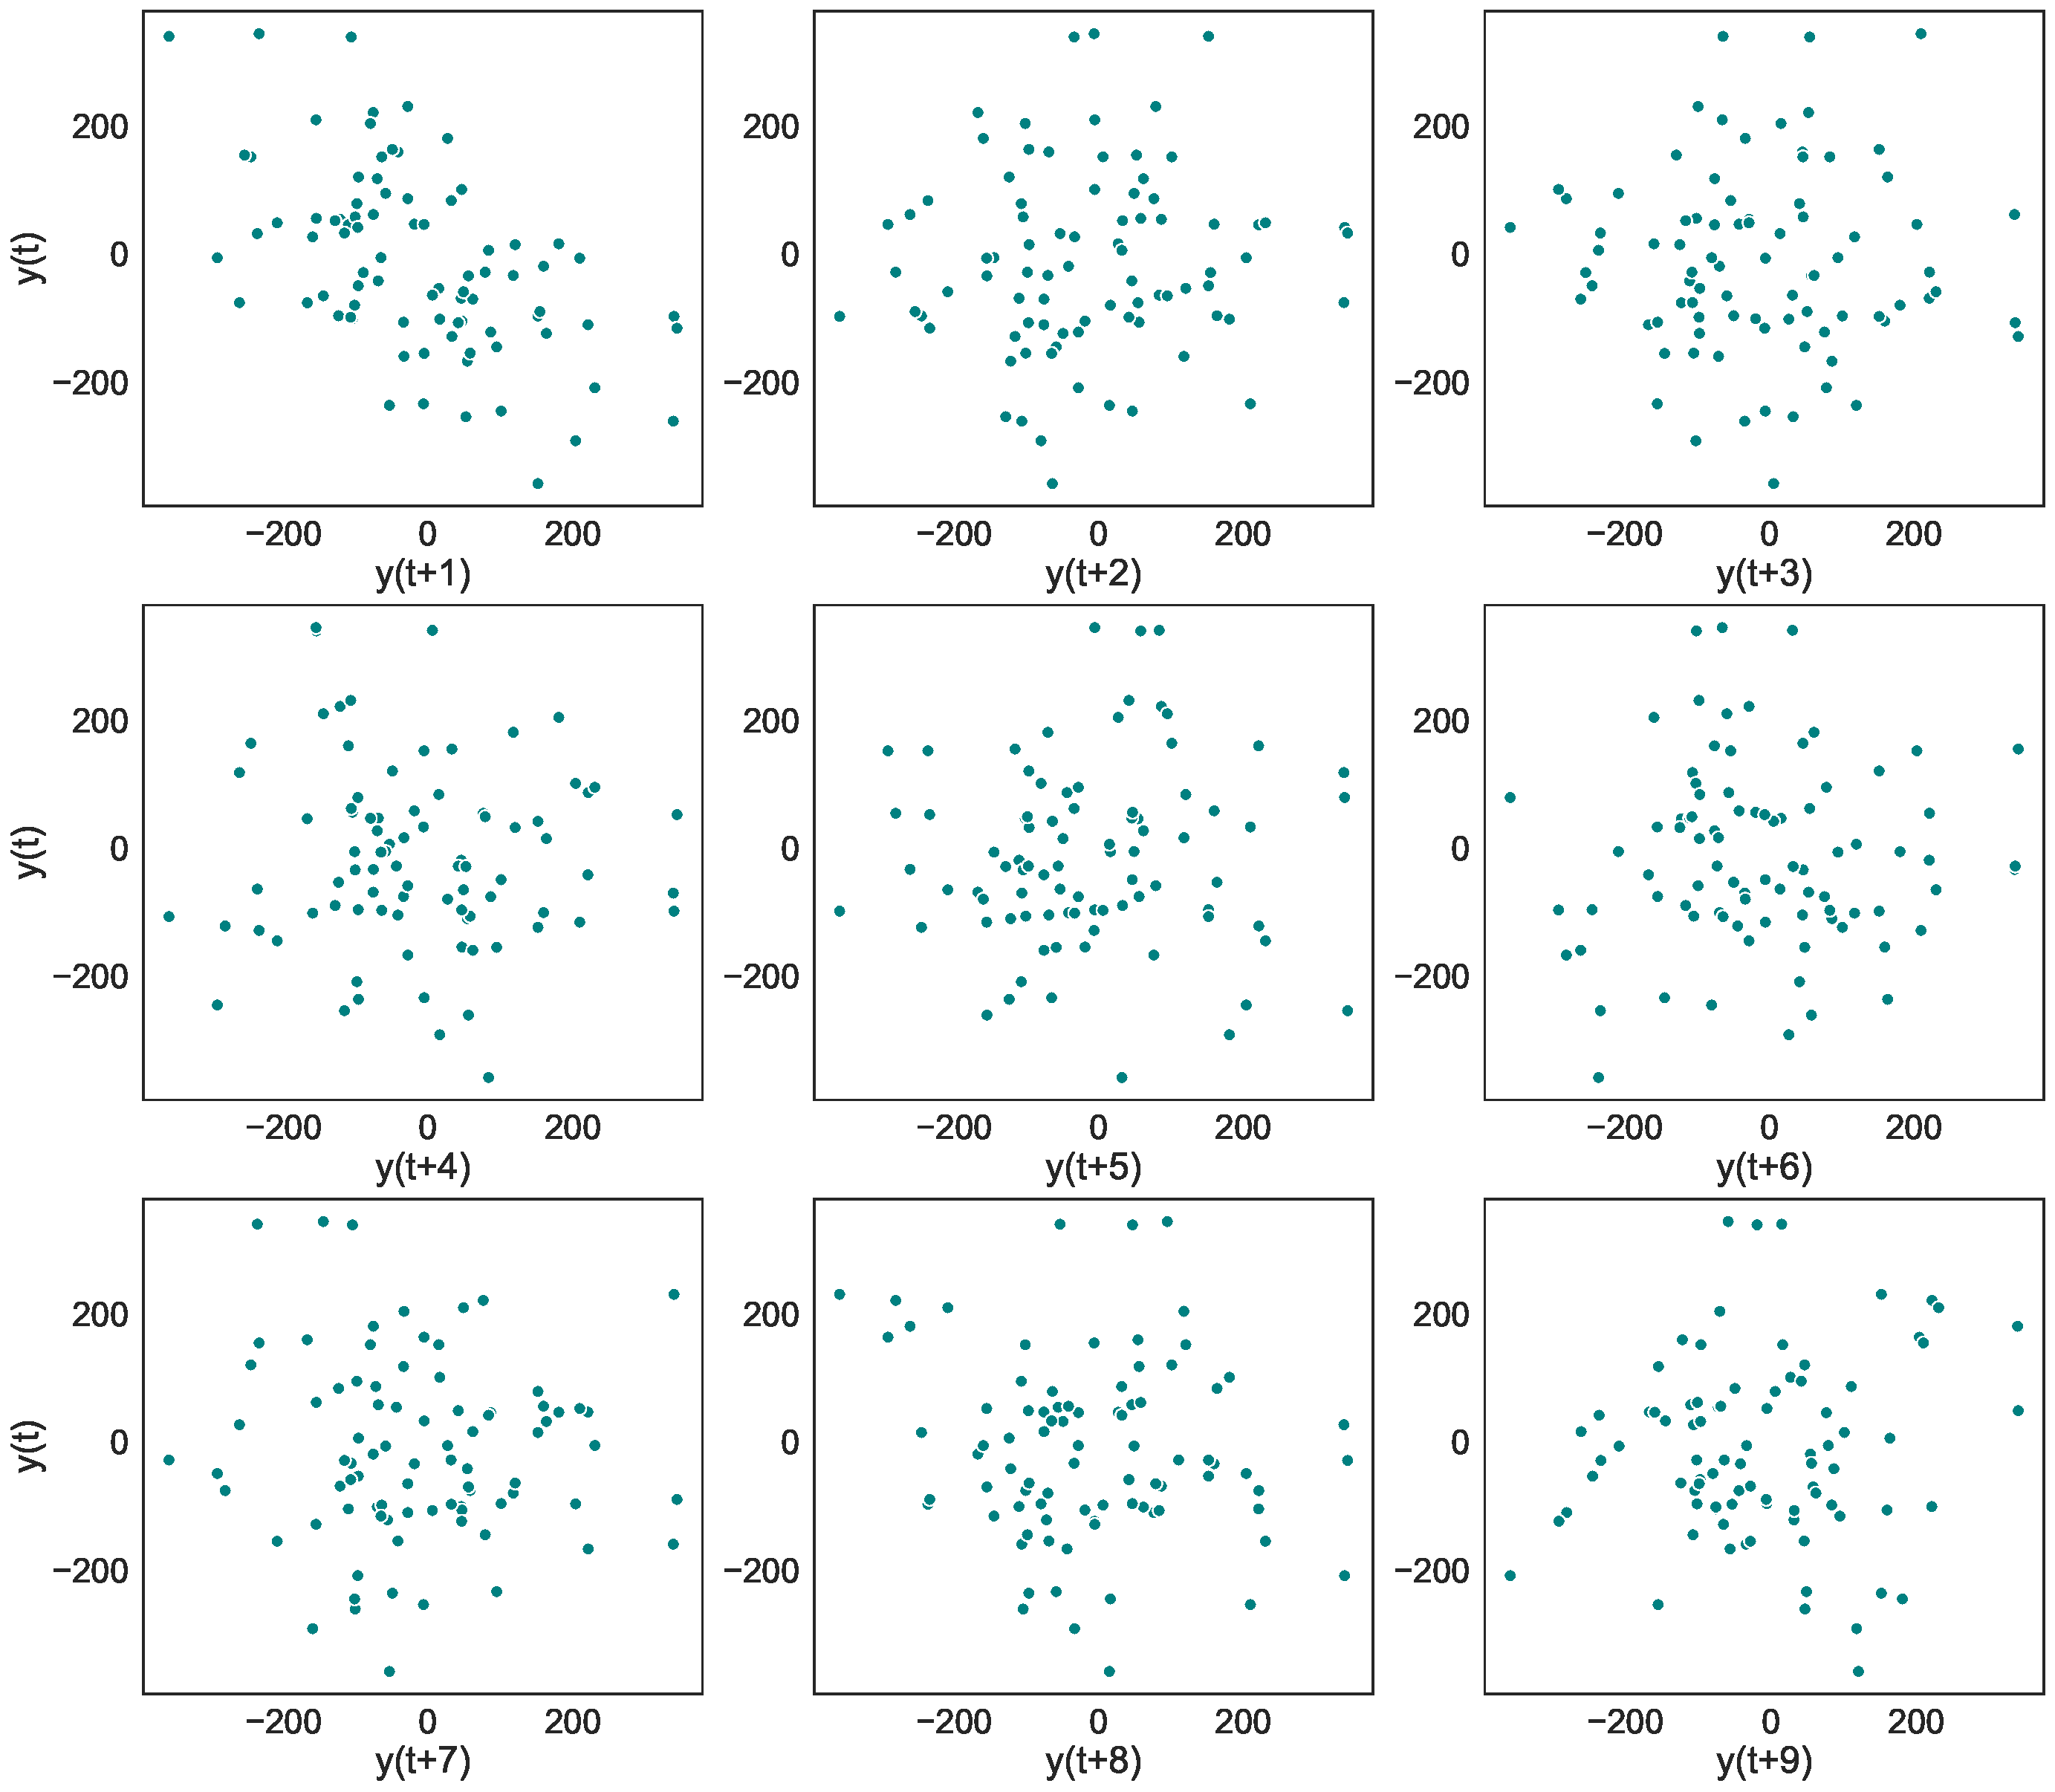
\includegraphics[width=1\textwidth]{../figs/joe_lag_plots.pdf}
\caption{Log plots for different values of $h$ (from 1 to 9). It is clear that there is a strong correlation with the previous day, even tough correlations decrease as we consider higher values of h, i.e. larger time shifts.}\label{fig:joe_lag_plots}
\end{figure}

\begin{figure}\centering
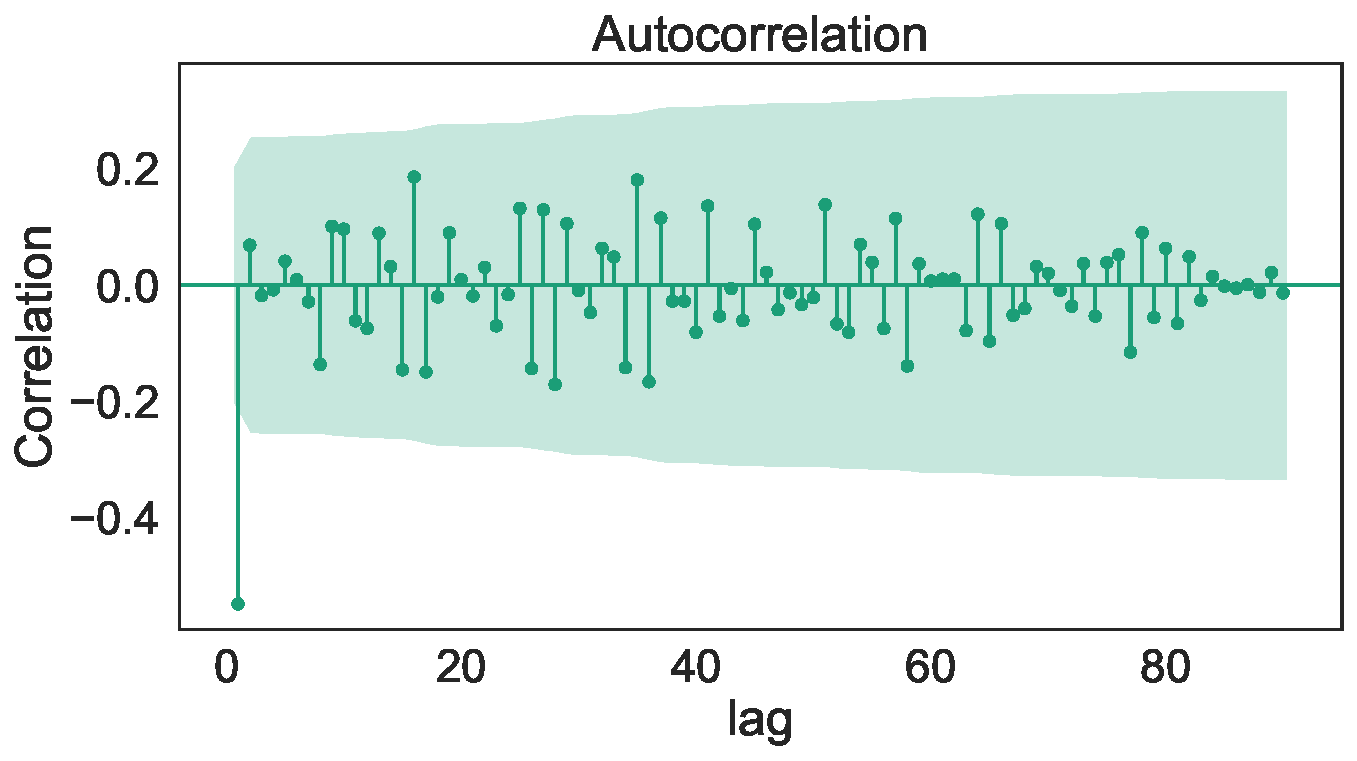
\includegraphics[width=0.7\textwidth]{../figs/joe_autocorr.pdf}
\caption{Autocorrelation plot for all the possible shifts. It provides the correlation coefficient between $y(t)$ and $y(t+h)$ for different shifts.}\label{fig:joe_autocorr}
\end{figure}



\section{Simulation analysis}
In this section we perform a simulation, by means of Python Random Number Generators (RNG), to study the statistical properties of two distributions, uniform and normal, with particular reference to the computation of confidence intervals.

\subsection{Uniform distribution}\label{sec:unif}
Let us consider $n$ iid data generated randomly and uniformly distributed: $x_i\sim \mathcal U ([0,1]), \,\, i = 0, \dots,N-1$. We aim to study the statistical properties of such distribution for different values of $n$, in order to exploit and test different metrics and tools.

\subsubsection{Simulation with n=48}
Let us first generate $n=48$ $iid$ $x_i\sim \mathcal U ([0,1])$, we can compute sample mean, sample standard deviation and 95\%-confidence interval for the mean as follows:
\begin{equation}
\mu_n = \frac{\sum_i^n x_i}{n},
\end{equation}
\begin{equation}
\sigma_n =\sqrt{ \frac{\sum_i^n (x_i-\mu_n)}{n-1}}.
\end{equation}
The CI for the mean, assuming that the Central Limit Theorem (CLT) holds, can be computed as:
\begin{equation}
\left[\mu_n- \eta \frac{s_n }{\sqrt{n}}}, \mu_n+\eta \frac{s_n }{\sqrt{n}}},\right]
\end{equation}
where:
\begin{equation}
s_n =\sqrt{ \frac{\sum_i^n (x_i-\mu_n)}{n}},
\end{equation}
and $\eta$ for a level $\gamma$ is such that:
\begin{equation}
\mathcal N_{0,1}(\eta)=\frac{1+\gamma}{2}.
\end{equation}
In Table \ref{tab:48} we report the results computed on the sample.

\begin{table}[]\centering
\begin{tabular}{llll}
Distribution       & $\mu_n$ & $\sigma_n$ & 95\% $CI_{\mu_n}}$ \\ \hline
$\mathcal U (0,1)$ & 0.55    & 0.27       & {[}0.47, 0.62{]}                   \\
$\mathcal N (0,1)$ & 0.18    & 1.12       & {[}-0.14, 0.51{]}                 
\end{tabular}
\caption{Mean, standard deviation and 95\% CI for a simulation with a sample of 48 elements, for both uniform and normal distribution.}\label{tab:48}
\end{table}

\subsubsection{Repetition of the experiment 1000 times}
We now repeat the same experiments, i.e. generation of 48 samples, independently 1000 times. We then compute the probability that the true value of the mean is not contained in the CI. Over 1000 trials, we observe that this event happens with 6\% probability, which is close to the 5\% we would expect since we fixed a confidence level of 95\%.
In Figure\ref{fig:mean_unif} we plot the distribution of the observed means, compared with the true mean, dashed line, while in Figure \ref{fig:meanci_unif} we plot the CI with the corresponding mean. From the latter, we can compare the true mean with the computed mean, in ascending order, and highlight when it falls into the computed CI.

\begin{figure} \centering
\begin{subfigure}{0.5\textwidth}
         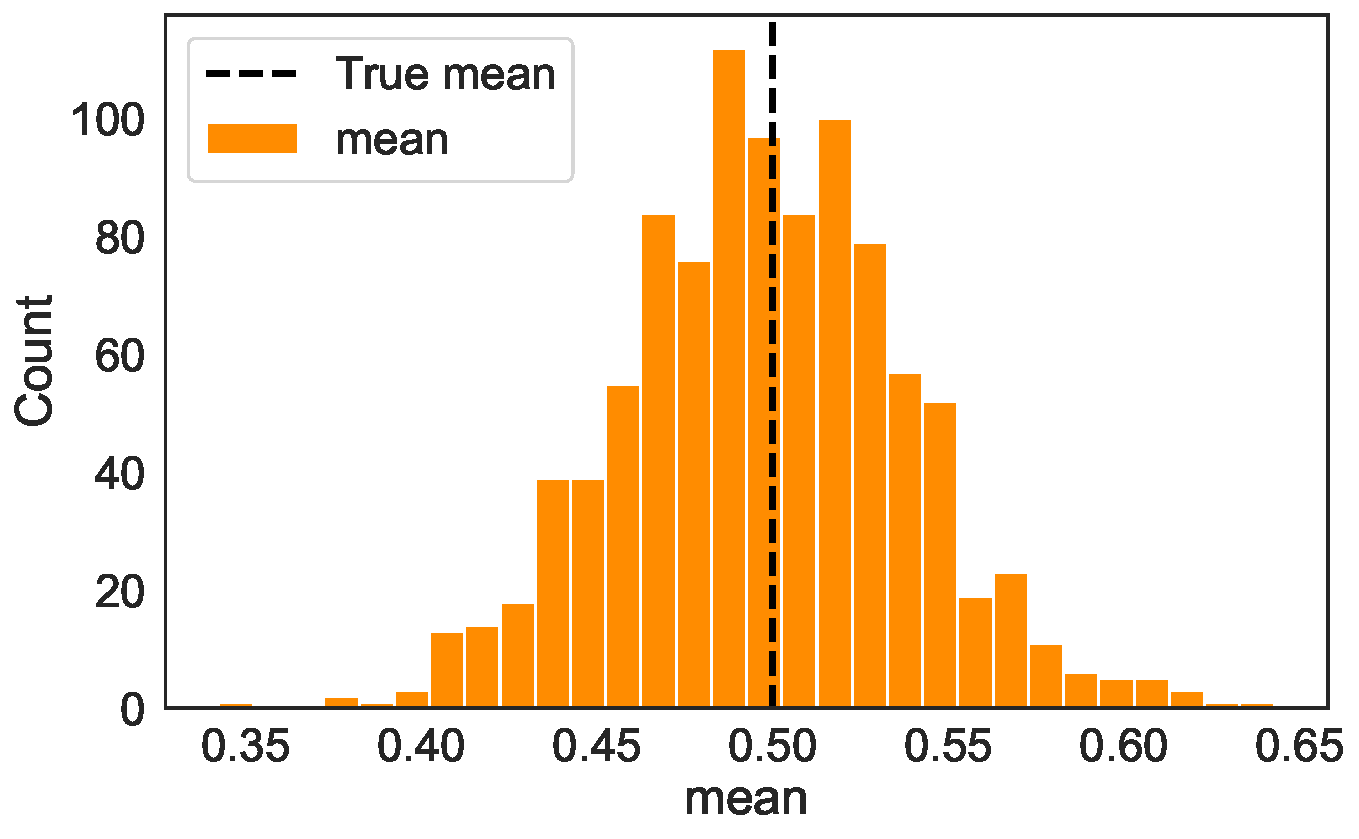
\includegraphics[width=\textwidth]{../figs/mean_distr_unif.pdf}
         \caption{Distribution of the observed means computed on a sample of 48 items, compared with the true mean, represented by the vertical dashed line.}\label{fig:mean_unif}
     \end{subfigure}
     \begin{subfigure}{0.45\textwidth}
         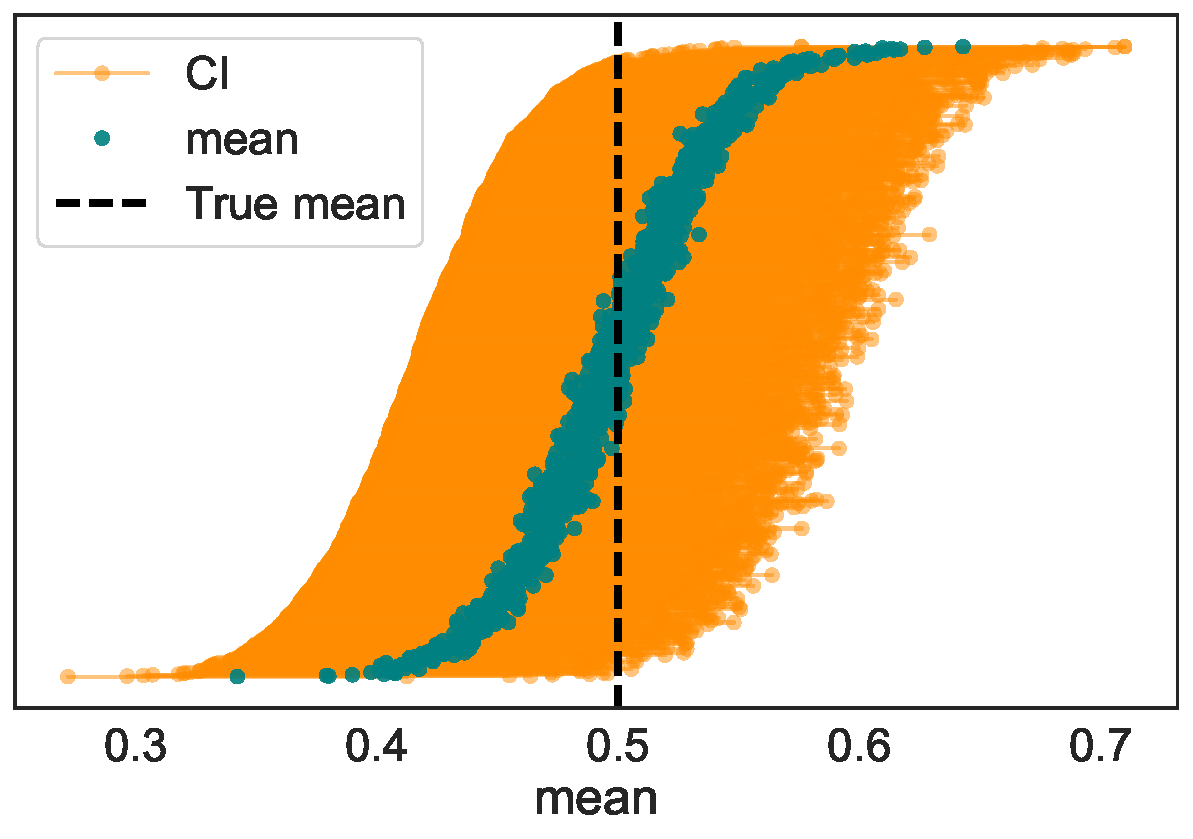
\includegraphics[width=\textwidth]{../figs/unif_mean_CI.pdf}
         \caption{ CI and corresponding sample mean, computed on 1000 datasets of 48 elements. The vertical dashed line represents the real mean, and it shows how many times it falls into the computed CI.}\label{fig:meanci_unif}
     \end{subfigure}
  \caption{Results concerning the generation of 1000 datasets, each of which is composed by 48 elements uniformly distributed in $[0,1]$.  }\label{fig:ci_unif_mean}
\end{figure}

\subsubsection{Comparison of results for different values of $n$}
Another interesting analysis consists of testing such statistical tools on a dataset of different sizes. In particular we generate $n$ $iid$ elements uniformly distributed in $[0,1]$ and for different values of $n$, we then compute the mean and the sample variance. Note that, in order to generate random numbers, we need to fix a seed for the pseudo RNGs, and we choose to do so in such a way that each dataset is made up by the same initial values and new data generated according to the new size of the set. This is due to the fact that we want to compare how the metrics are influenced by the size of the datasets, thus we decide to work with at least the same initial part of data.\par
In Figure \ref{fig:N_unif} we show the accuracy of the mean, computed as logarithm of the inverse $\epsilon=\mu_{data}-\mu_{real}$, and the CI of the variance for different values of $n$. For what concerns the comparison of the sample mean with the real value, in Figure \ref{fig:N_unif_acc} we observe that the accuracy of the mean is subjected to oscillation, with a general increasing trend as $n$ increases. In particular it gets more stable for high values of $n$. On the other hand, in Figure \ref{fig:N_unif_var} we show the variance and its CI for different values of $n$. The main outcome is that, as we increase the size of the dataset, our uncertainty on the estimate of the variance decreases.

\begin{figure} \centering
\begin{subfigure}{0.45\textwidth}
         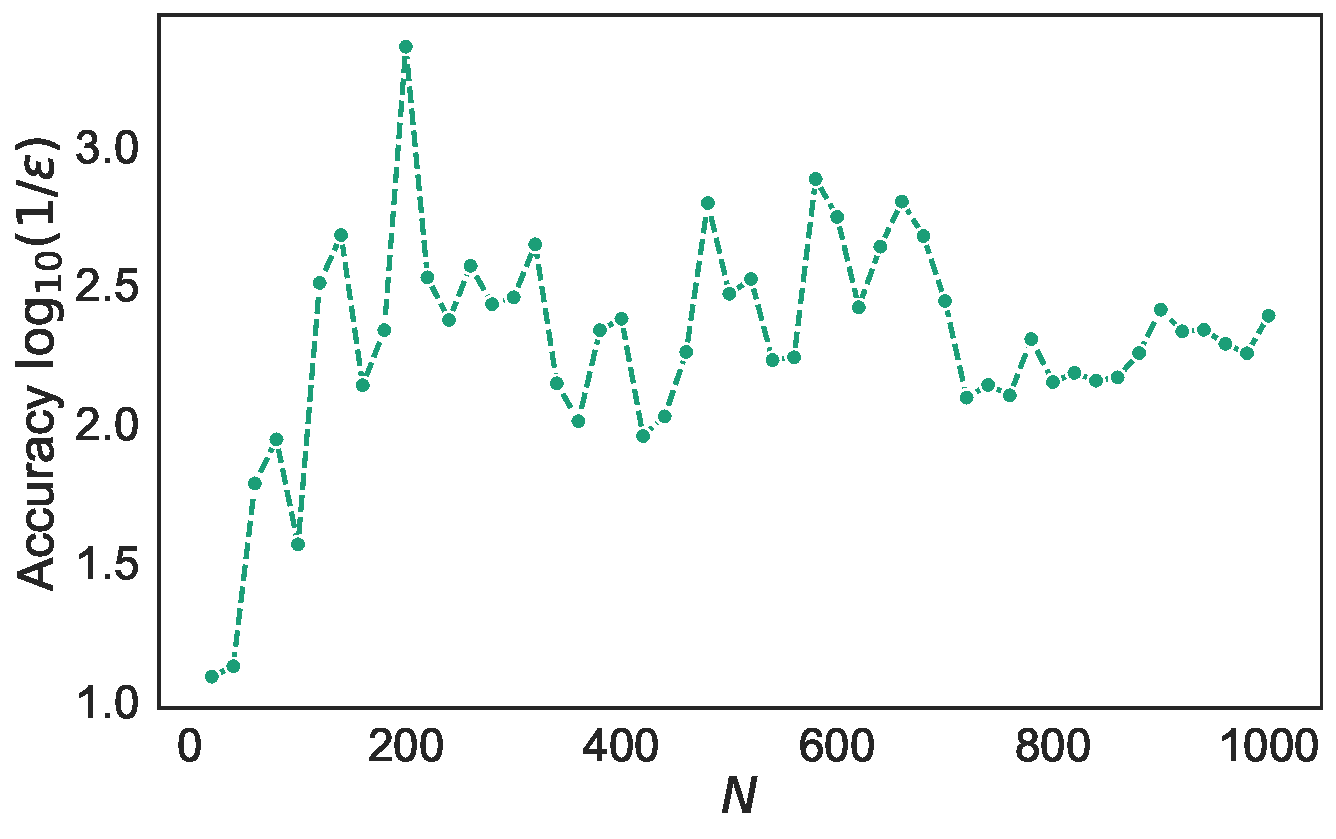
\includegraphics[width=\textwidth]{../figs/unif_mean_accuracy.pdf}
         \caption{Accuracy of the estimation of the mean for different sizes of the dataset. We observe oscillations, with a general increasing trend, as $n$ increases, in particular the curve gets more stable for high values of $n$.}\label{fig:N_unif_acc}
     \end{subfigure}
     \begin{subfigure}{0.5\textwidth}
         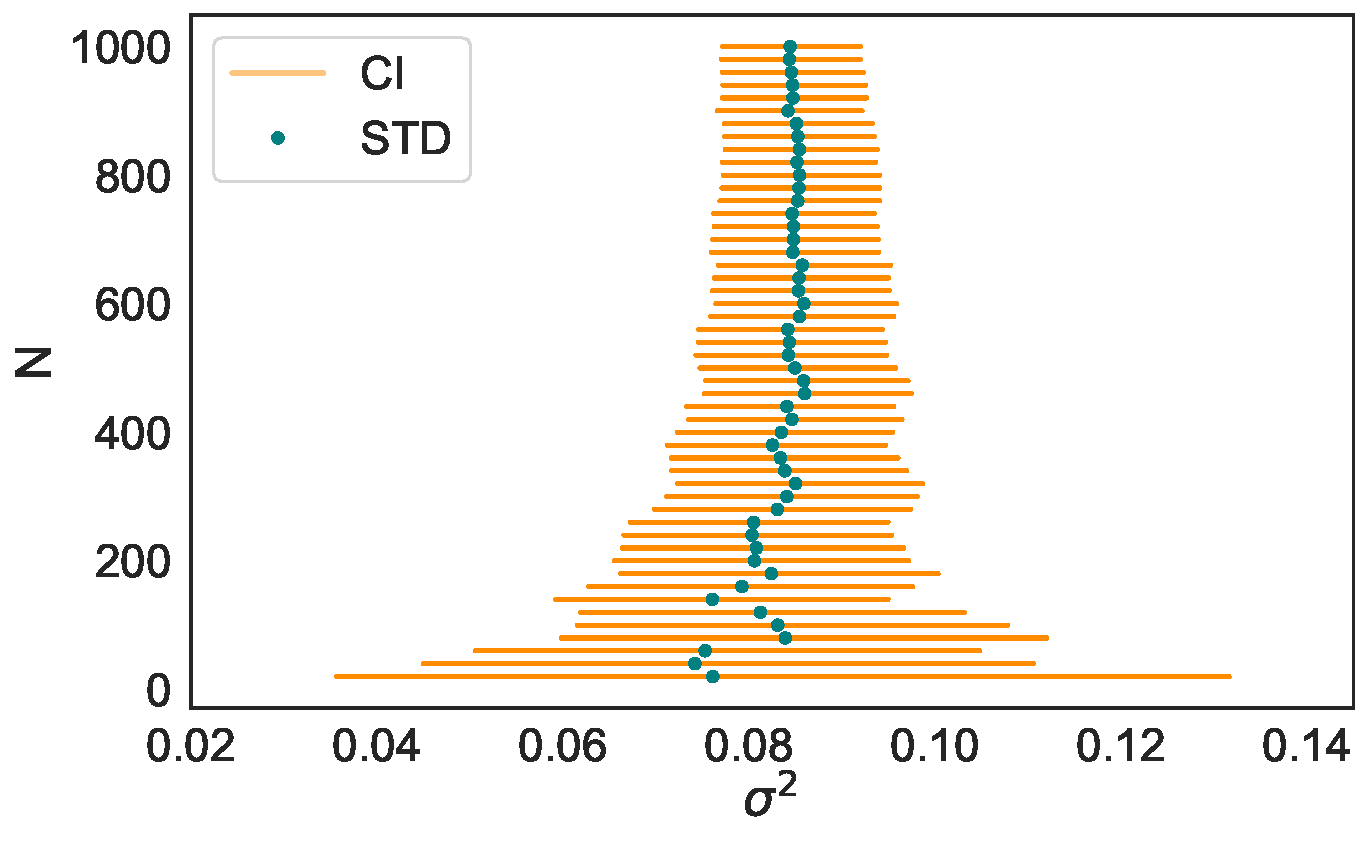
\includegraphics[width=\textwidth]{../figs/unif_variance_CI.pdf}
         \caption{Variance and its CI for different values of $n$. As we increase the size of the dataset, our uncertainty on the estimate of the variance decreases.}
         \label{fig:N_unif_var}
     \end{subfigure}
  \caption{Accuracy of the mean, computed as $\log(1/\epsilon)$ where $\epsilon=|\mu_n-\mu_{real}|$, and the CI of the variance for different values of $n$}\label{fig:N_unif}
\end{figure}

\subsubsection{Prediction intervals}
Finally, we generate a series of 1000 random numbers and we compute the corresponding prediction intervals with two methods: with bootstrap approximation and with the standard method based on order statistic. The first is based on computing the quantiles, given a certain confidence level, on the observed statistic, while the second relies on the assumption that data are iid. In particular, given a series of $n$ $iid$ data $\{X_i\}_{i=0,\dots,n}$, and its order statistic $\{X^n_{(i)}\}}_{i=0,\dots,n}$, prediction interval can be computed as follows:
\begin{equation}
\left[ X^n_{\lfloor(n+1)\alpha/2\rfloor}, X^n_{\lfloor(n+1)(1-\alpha/2)\rfloor}\right],
\end{equation}
where $\alpha$ must satisfy $\alpha \geq \frac{2}{n+1}$ and, fixed a level $\gamma$, it is computed as $\gamma=1-\alpha$. In Table \ref{tab:pi} we report results for the two different methods.


\begin{table}[]\centering
\begin{tabular}{lll}
Distribution       & $PI $ Order statistic & $PI $ Bootstrap  \\ \hline
$\mathcal U (0,1)$ & {[}0.02, 0.98{]}       & {[}0.03, 0.98{]}  \\
$\mathcal N (0,1)$ & {[}-1.98, 1.96{]}      & {[}-1.97, 1.95{]}
\end{tabular}\caption{CI computed with the standard method for $iid$ data, based on order statistic, and with bootstrap. We consider two datasets of 1000 elements, one with normal and one with uniform distribution. }\label{tab:pi}
\end{table}



\subsection{Normal distribution}
Let us now consider $n$ iid data generated randomly and normally distributed with zero mean and unitary variance: $x_i\sim \mathcal N (0,1)$. We will repeat the analysis as in Section \ref{sec:unif}.

\subsubsection{Simulation with n=48}
We first consider a dataset of 48 elements and compute sample mean, standard deviation and mean CI with the same formulas exploited in Section \ref{sec:unif}. Results are reported in Table \ref{tab:48}.


\subsubsection{Repetition of the experiment 1000 times}
We then generate 1000 independent dataset, each of which is composed by 48 elements. 

The probability that the true value of the mean does is not contained in the CI is 6\%, while we would expect 5\% since we fixed a confidence level of 95\%. This is probably due to approximations introduced in the simulation itself and by the randomness of the system.
In Figure \ref{fig:mean_norm} we plot the distribution of the observed means and the corresponding true value, while in Figure \ref{fig:meanci_norm} we exhibit the CI and all the sample means. The latter allows to compare the true mean with the computed mean and to observe when the true value falls into the simulation CI.

\begin{figure} \centering
\begin{subfigure}{0.5\textwidth}
         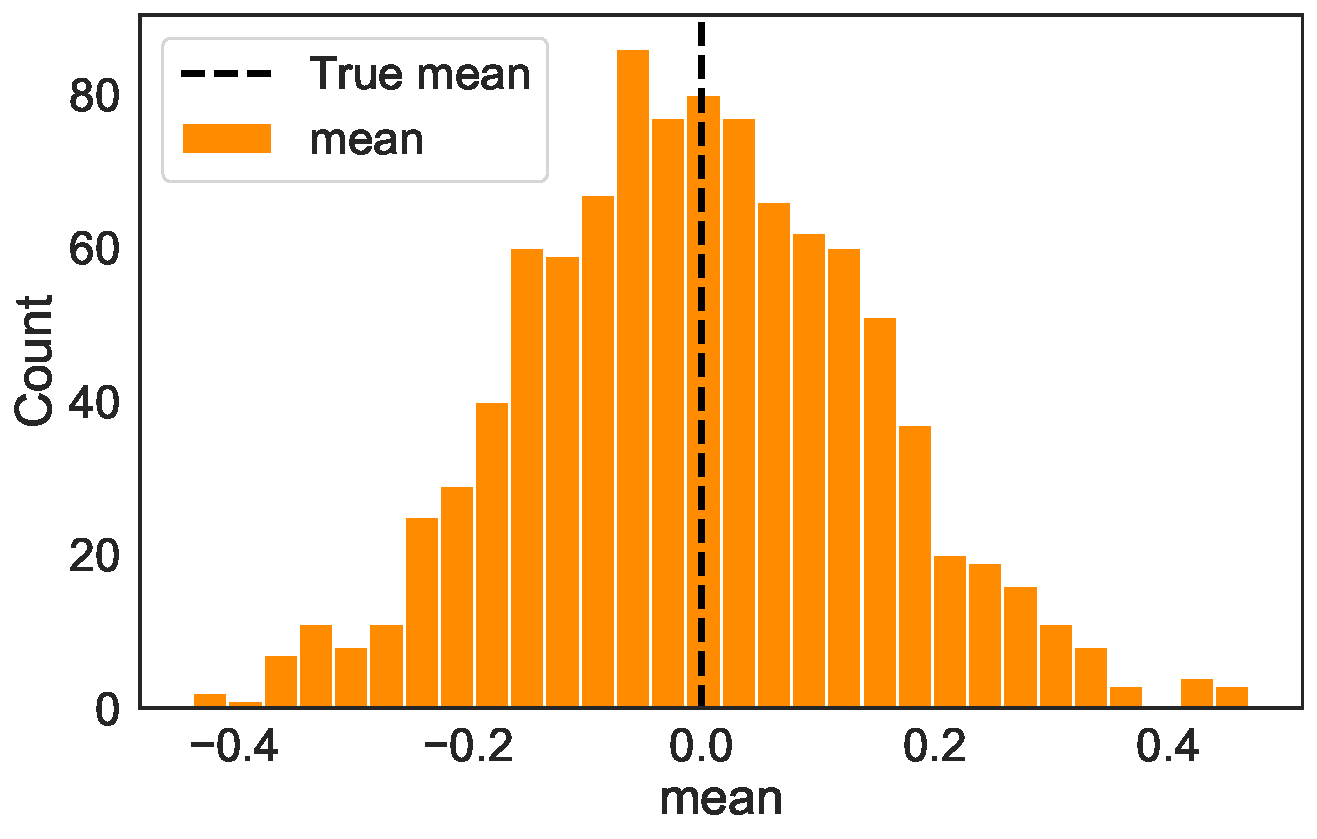
\includegraphics[width=\textwidth]{../figs/mean_distr_norm.pdf}
         \caption{Distribution of the observed means computed on a sample of 48 items, compared with the true mean, represented by the vertical dashed line.}\label{fig:mean_norm}
     \end{subfigure}
     \begin{subfigure}{0.45\textwidth}
         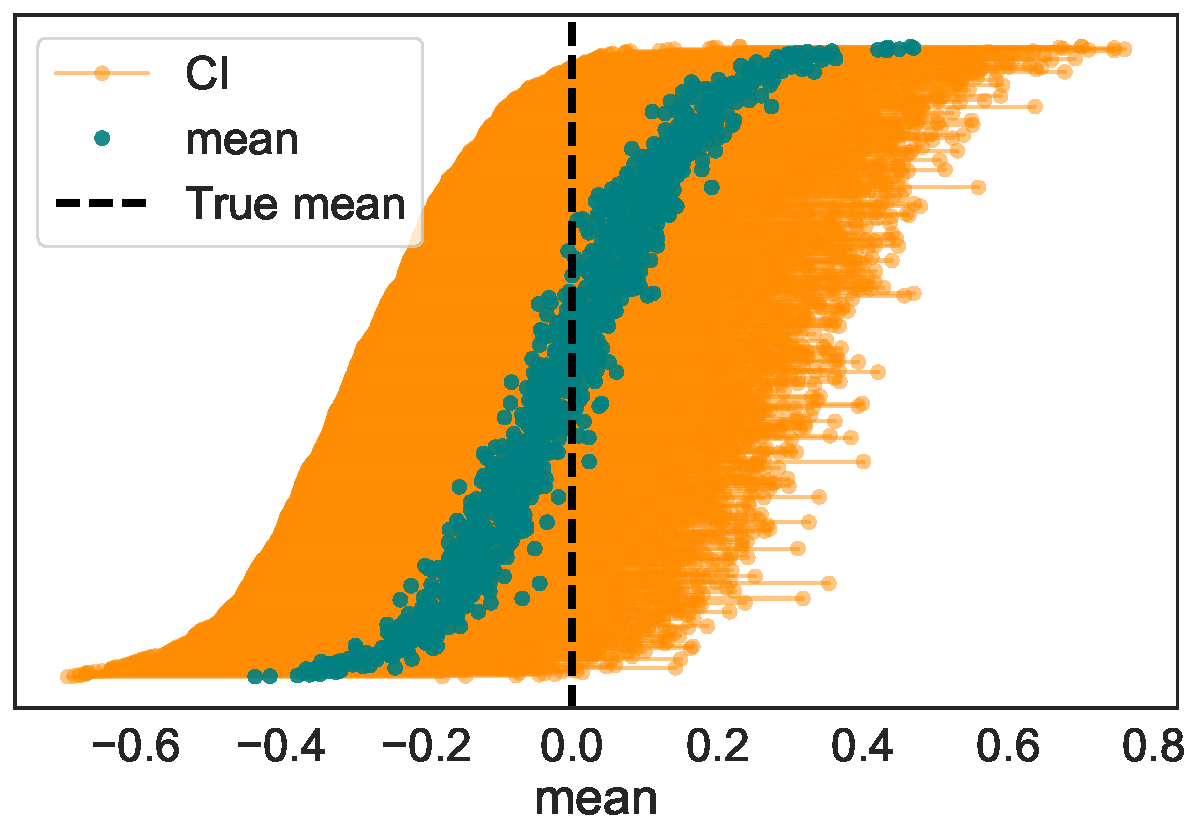
\includegraphics[width=\textwidth]{../figs/norm_mean_CI.pdf}
         \caption{CI and corresponding sample mean, computed on 1000 datasets of 48 elements. The vertical dashed line represents the real mean, and it shows how many times it falls into the computed CI.}\label{fig:meanci_norm}
     \end{subfigure}
  \caption{Results concerning the generation of 1000 datasets, each of which is composed by 48 elements normally distributed with zero mean and unitary variance.  }\label{fig:ci_norm_mean}
\end{figure}

\subsubsection{Comparison of results for different values of $n$}
Eventually, we can generate datasets of different sizes, with the same structured exposed in Section \ref{sec:unif}.  

In Figure \ref{fig:N_norm} we report the accuracy of the mean and rhe CI of the variance for different dataset sizes. The accuracy, see Figure \ref{fig:N_norm_acc}, has an irregular increasing behaviour for $n<400$, while it gets stable for larger datasets. Figure \ref{fig:N_norm_var} shows the variance and its CI, the main outcome is uncertainty on the estimate of the variance decreases for larger values of $n$.

\begin{figure} \centering
\begin{subfigure}{0.45\textwidth}
         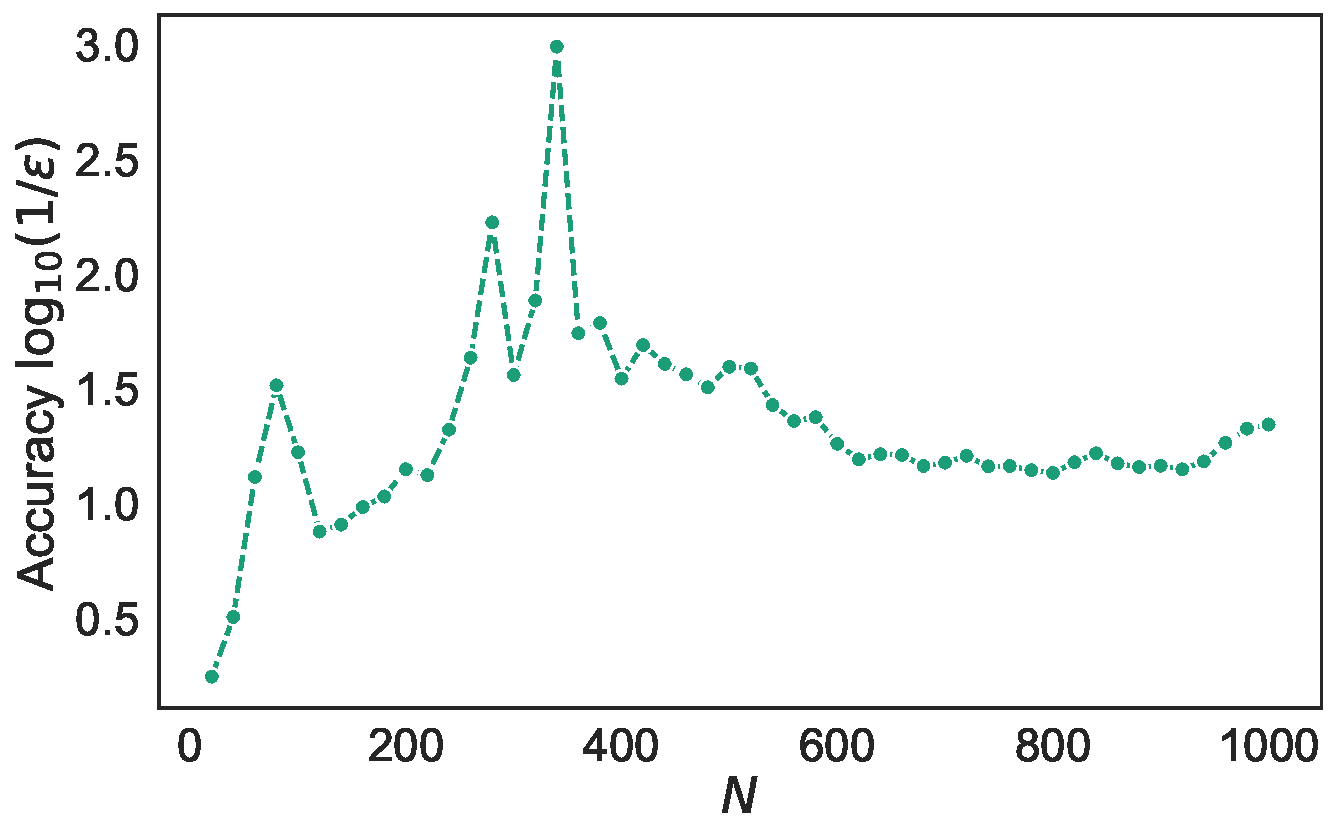
\includegraphics[width=\textwidth]{../figs/norm_mean_accuracy.pdf}
         \caption{Accuracy of the estimation of the mean for different sizes of the dataset. We observe an irregular increasing trend, in particular the curve gets more stable for high values of $n$.}\label{fig:N_norm_acc}
              \end{subfigure}
     \begin{subfigure}{0.5\textwidth}
         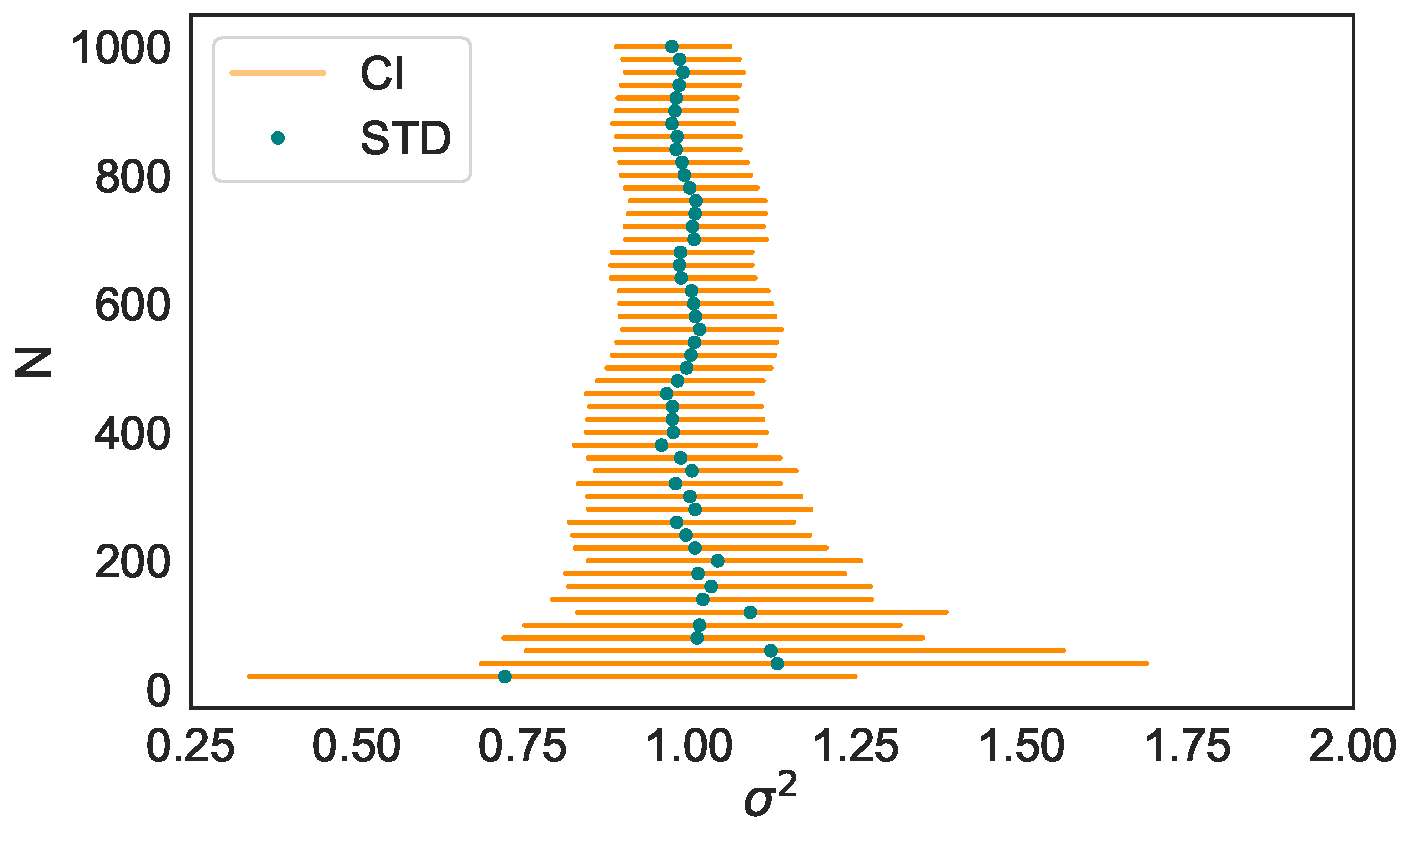
\includegraphics[width=\textwidth]{../figs/norm_variance_CI.pdf}
         \caption{Variance and its CI for different values of $n$. As we increase the size of the dataset, our uncertainty on the estimate of the variance decreases.}
         \label{fig:N_norm_var}
     \end{subfigure}
  \caption{Accuracy of the mean, computed as $\log(1/\epsilon)$ where $\epsilon=|\mu_n-\mu_{real}|$, and the CI of the variance for different values of $n$}\label{fig:N_norm}
\end{figure}


\subsubsection{Prediction intervals}
Finally, we compute the prediction intervals with order statistic and bootstrap on a sample of 1000 $iid$ normally distributed data, the procedure is analogue to the one described in reference to uniform distributed data. Table \ref{tab:pi} report the PI for both the methods, which provide slightly different results.



\section{Order statistic}
Let us consider a dataset of $n$ $iid$ elements, uniformly distributed in $[0,1]$ and the corresponding ordered statistics, to whom we refer as:
\begin{equation}
X_{(1)}^n, \dots, X_{(n)}^n \quad \text{such that} \quad X_{(i)}^n< X_{(j)}^n\,\, \forall i<j.
\end{equation}
Let us consider first of all the general case in which data are distributed with a generic CDF $F(x)$, for a fixed value $x$ the probability that a certain data $X_{(j)}^n$ in the ordered sequence is smaller than $x$ is equal to the joint probability that $n- j$ elements are $> x$ and  $j$ are smaller. This has to be considered for all  for all the possible combinations of  the last $n - j$ elements. Recalling that, fixed $x$, the probability of being smaller is given by the CDF $F_j(x)= P(X_j\leq x))$ and the process "being smaller or larger than $x$" is binomial with probability $F(x)$, we can write the CDF of the order statistic as follows:
\begin{equation}
F_k^n (x)=\sum_{i=k}^{n}\binom{n}{i}(1-F(x))^{n-i}(F(x))^i.
\end{equation}
Going back to the uniform distribution, for which $F(x)=x$, we have:
\begin{equation}
F_k^n (x)=\sum_{i=k}^{n}\binom{n}{i}(1-x)^{n-i}(x)^i.
\end{equation}
To retrieve the density function we just derive the previous equation, after manipulation we find:
\begin{equation}
f_k^n(x)= n\binom{n-1}{k-1}(1-x)^{n-k}x^{k-1}.
\end{equation}
The mean value is then computed as:
\begin{equation}\begin{split}
<X_{k}>=& n\binom{n-1}{k-1} \int_0^1(1-x)^{n-k}x^{k} \,\, dx \\
=& - n\binom{n-1}{k-1} \sum_{i=0}^k \frac{(n-k)! k!}{(n-k+1+i)! (k-i)!}(1-x)^{n-k+1+i}x^{k-i}\Big|_{x=0}^{x=1},
\end{split}\end{equation}
where in the second equality we used a multiple integration by parts. Since for $x=1$ the only non null value is for $i=-n+k-1$ and for $x=0$ the only non null value is for $i=k$. Nevertheless, $i=-n+k-1$ does not correspond to a valid value for $i$ since it must be greater than 0 and lower than $k$, but  $i=-n+k-1>0 \Rightarrow k>n+1$, but by construction $k\geq n$. Therefore, we only consider $i=k$ for $x=0$, and obtain:
\begin{equation}\begin{split}
<X_{k}>=&n\binom{n-1}{k-1}  \frac{(n-k)! k!}{(n+1)! }\\
=&\frac{n(n-1)! }{(n-k)! (k-1)!} \frac{(n-k)! k!}{(n+1)! }\\
=& \frac{k}{n+1}
\end{split}\end{equation}



\end{document}

